% =======================  C�digo do Cap�tulo 1. ==================================
%Se precisar gerar outros cap�tulos use a op��o %Arquivo > Salvar Como e salve o novo arquivo com outro nome. Assim como este arquivo, %sugerimos seguir com a mesma linha de racioc�nio e salvar como capitulo2 e assim por diante. %N�O SE ESQUE�A DE COLOCAR NO ARQUIVO MODELOIFES.TEX O COMANDO %\INSERT{NOMEDOARQUIVODOCAP�TULO}. =============================


\begin{titlepage}


\setcounter{page}{13} % Define qual � o n�mero da primeira p�gina do cap�tulo

\chapter{\textbf{CRONOGRAMA}} % Este comando � utilizado para criar cap�tulos
\onehalfspacing % Espa�amento de 1,5

\vspace{0.5cm} % Aqui � configurado os 2 espa�os de 1,5
	
\begin{figure}[!h]
	\centering
	\caption{Cronograma parte 1}
	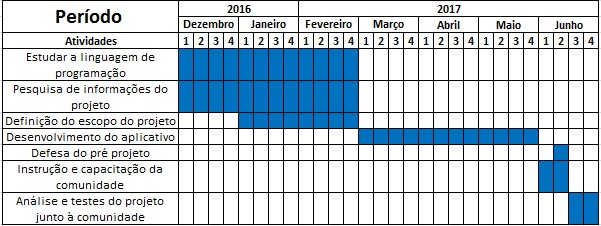
\includegraphics[width=1.0\linewidth]{imagens/cronograma_parte_1.jpg}
	\caption*{Fonte: Pr�pria}
\end{figure}	

\begin{figure}[!h]
	\centering
	\caption{Cronograma parte 2}
	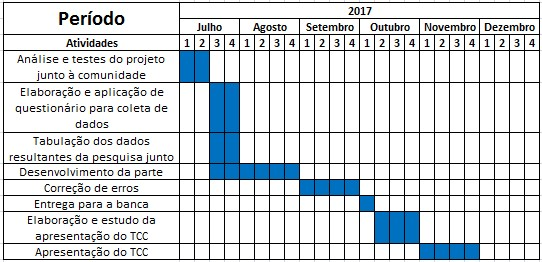
\includegraphics[width=1.0\linewidth]{imagens/cronograma_parte_2.jpg}
	\caption*{Fonte: Pr�pria}
\end{figure}	


\end{titlepage}